\section{Additional Experiment 1 simulations with kernel nuisance estimators}
\label{appendix::exp1_kernel_sensitivity}

We repeated the singly consistent simulations from Experiment~1 with the same
data-generating distribution, sample-splitting scheme, seed convention,
estimators, and inferential procedures, changing only the nuisance estimator
used for the component deliberately set to be misspecified or estimated at a
slow rate.
In the first additional run, the misspecified main-term logistic regression used
in Experiment~1 is replaced by a misspecified Nadaraya-Watson kernel regression
that uses \(W_1\) and omits the binary covariate \(W_2\). In the second
additional run, the same stratified Nadaraya-Watson kernel regression is used
with the suboptimal bandwidth rule \(h_m=m^{-0.025}\), where \(m\) is the
training-stratum sample size, rather than bandwidth selection by
cross-validation. We report the complete cells with
\(n \in \{250,500,750,1000,2000,3000,4000,5000\}\), using 500 Monte Carlo
replicates per cell.

Figure~\ref{fig::exp1_slow_kernel_appendix} gives the results for the
slow-bandwidth kernel nuisance estimator. The empirical pattern is similar to
that in Figure~\ref{fig::exp1}: IC-DML has low empirical bias and coverage near
the nominal 95\% level in both singly consistent settings, while AIPW has larger
bias or lower coverage when the slow bandwidth rule is used.

\begin{figure}[tbp]
     \centering
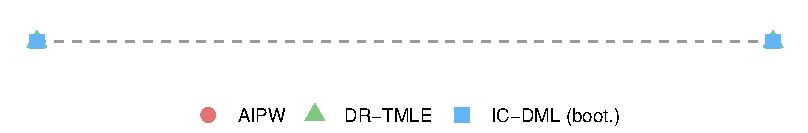
\includegraphics[width=0.5\linewidth]{newplots/appendix_exp1_kernel_sensitivity_legend.pdf}

    \begin{subfigure}[b]{\linewidth}
    \centering
    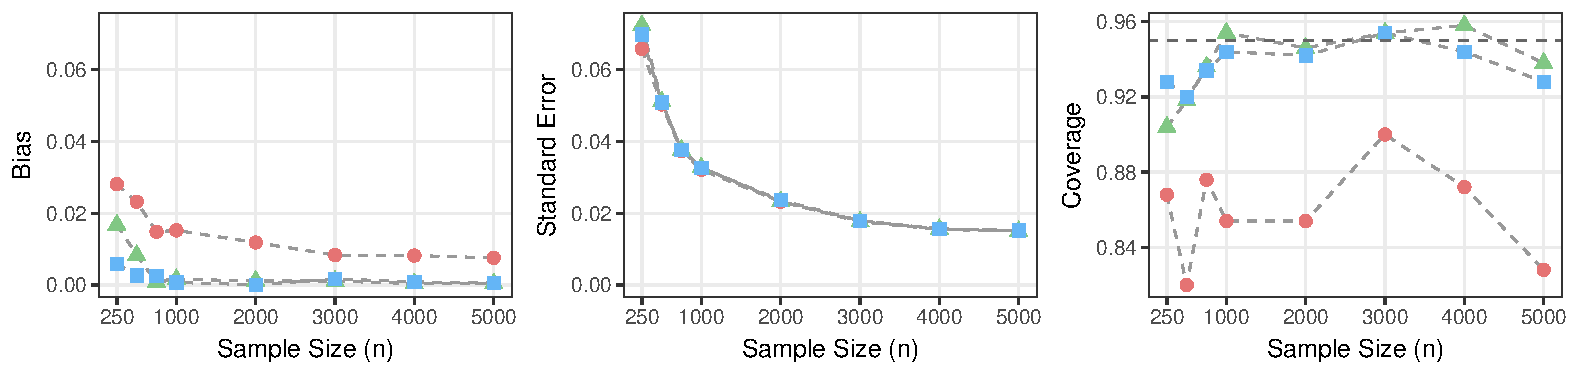
\includegraphics[width=\linewidth]{newplots/appendix_exp1_slow_kernel_misp3.pdf}
    \subcaption{Only outcome regression is estimated consistently.}
    \end{subfigure}
    \begin{subfigure}[b]{\linewidth}
    \centering
    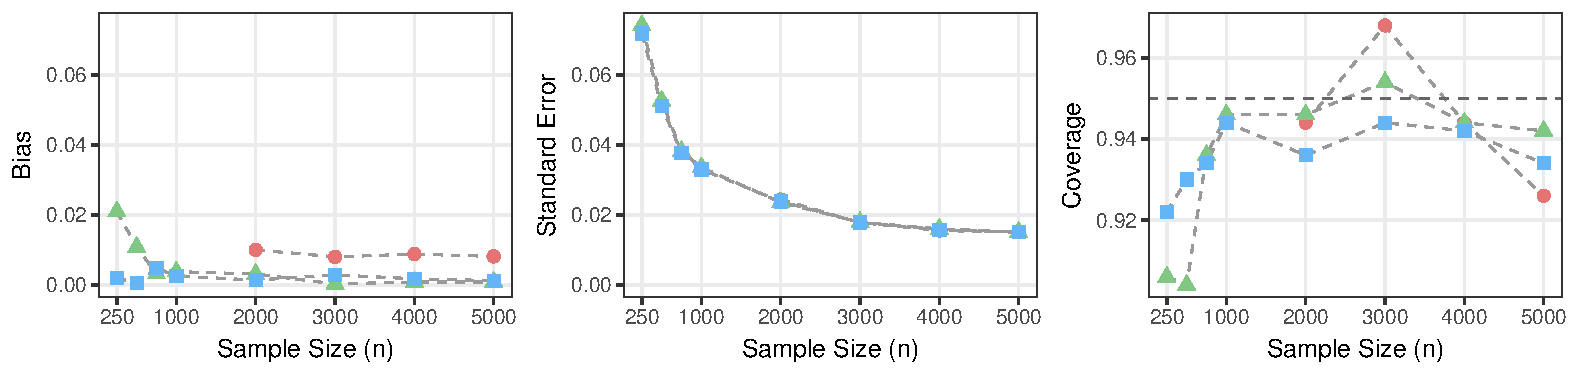
\includegraphics[width=\linewidth]{newplots/appendix_exp1_slow_kernel_misp2.pdf}
   \subcaption{Only propensity score is estimated consistently.}
    \end{subfigure}
\caption{Additional Experiment~1 results using a slow-bandwidth kernel nuisance estimator with \(h_m=m^{-0.025}\). Bias, standard error, and 95\% confidence interval coverage are shown for AIPW, DR-TMLE, and IC-DML. IC-DML uses the bootstrap interval; AIPW and DR-TMLE use Wald intervals.}
       \label{fig::exp1_slow_kernel_appendix}
\end{figure}

Figure~\ref{fig::exp1_one_variable_kernel_appendix} gives the results when the
misspecified logistic regression is replaced by the one-variable kernel
regression. When only the propensity score is consistently estimated, IC-DML has
low empirical bias and coverage close to nominal over the displayed sample
sizes. When only the outcome regression is consistently estimated, the
empirical bias of calibrated DML and DR-TMLE is below that of AIPW from
\(n=1000\) onward; the largest departures from nominal IC-DML coverage occur at
the two smallest sample sizes. The ordering is similar to
Figure~\ref{fig::exp1}, apart from lower IC-DML coverage at the two smallest
sample sizes in the outcome-regression-consistent setting.

\begin{figure}[tbp]
     \centering
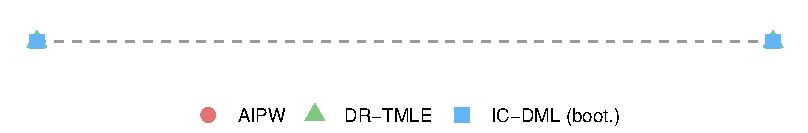
\includegraphics[width=0.5\linewidth]{newplots/appendix_exp1_kernel_sensitivity_legend.pdf}

    \begin{subfigure}[b]{\linewidth}
    \centering
    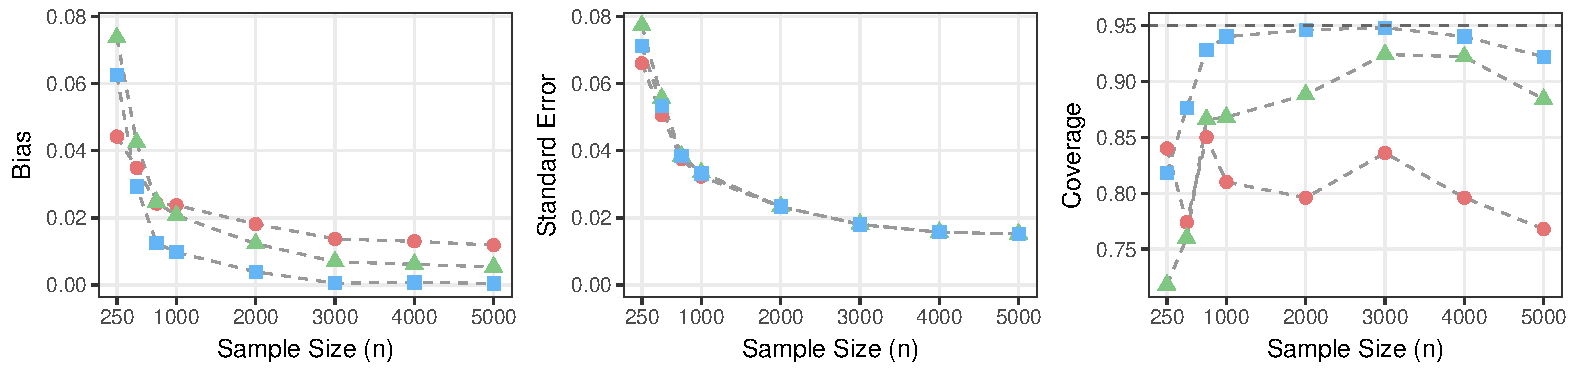
\includegraphics[width=\linewidth]{newplots/appendix_exp1_one_variable_kernel_misp3.pdf}
    \subcaption{Only outcome regression is estimated consistently.}
    \end{subfigure}
    \begin{subfigure}[b]{\linewidth}
    \centering
    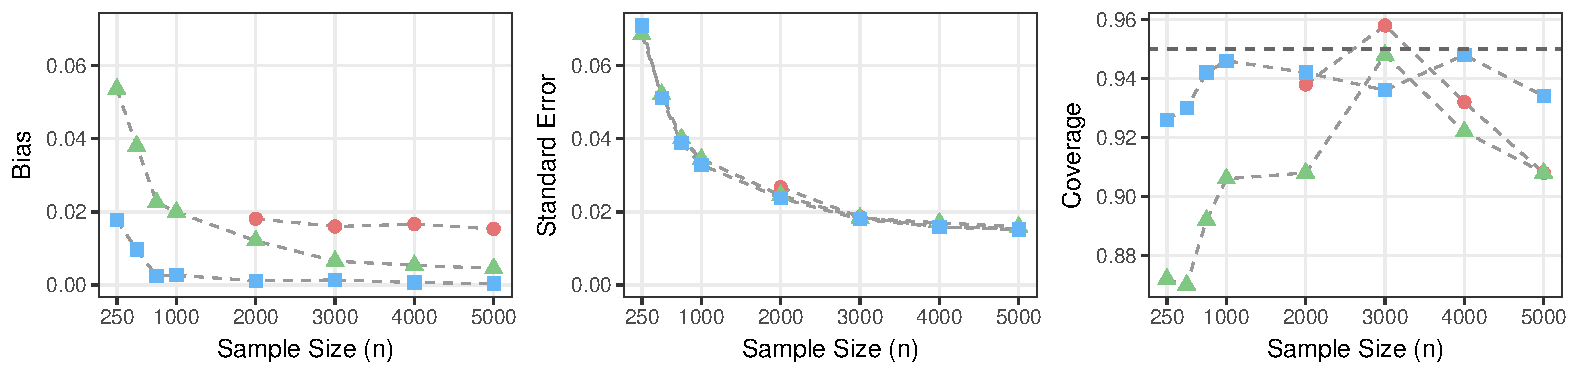
\includegraphics[width=\linewidth]{newplots/appendix_exp1_one_variable_kernel_misp2.pdf}
   \subcaption{Only propensity score is estimated consistently.}
    \end{subfigure}
\caption{Additional Experiment~1 results using a misspecified one-variable kernel nuisance estimator that uses \(W_1\) and omits \(W_2\). Bias, standard error, and 95\% confidence interval coverage are shown for AIPW, DR-TMLE, and IC-DML. IC-DML uses the bootstrap interval; AIPW and DR-TMLE use Wald intervals.}
       \label{fig::exp1_one_variable_kernel_appendix}
\end{figure}

In the outcome-misspecified panels, plotted AIPW points with empirical standard
error above 0.1 or absolute bias above 0.1 are omitted from the displayed curves
so that the common axes show the range of the other plotted points. These rows
are retained in the simulation summary files.
